\section{Anwendersicht}
Für die Anwendersicht wurden zwei Applikationen erstellt. Zum einen eine Mobile Applikation und zum anderen eine Web Applikation. Die Mobile Applikation wurde für das Betriebssystem Android in AndroidStudio entwickelt. Die Web Applikation wurde mit Hilfe eines Bootstrap Templates erstellt. Beide Applikationen verwenden die Bibliothek Paho um mit der MOM zu Interagieren.  
\subsection{Andriod-APP}
Die Android Applikation soll eine Wetter Applikation sein, dafür soll sie verschiedene Wetterdaten anzeigen können. Dazu wurde zu beginn des Projektes festgelegt, welche Daten Anzeigt werden  sollen. Diese können in zwei Kategorien unterschieden werden. Zum einen das Tageswetter und zum anderen die Wochenvorhersage. Unter das Tageswetter fallen die folgenden Punkte: 
\begin{itemize}
\item das Tageswetter als großes Icon
\item die momentane Temperatur in $^\circ$C
\item das genaue Wetter in Wörtern
\item der Standort
\item das Datum mit Uhrzeit
\item die Windgeschwindigkeit in km/h
\item die Windrichtung mit Hilfe einer grafischen Anzeige
\item die Regenwahrscheinlichkeit in \%
\end{itemize}  
Bei der Wettervorhersage für eine Woche ergeben sich nachfolgende Punkte
\begin{itemize}
\item die Wochentage ab dem nachfolge Tag des Tageswetters
\item ein kleines Wettericon
\item die Tagesmaximaltemperatur in $^\circ$C mit der Schriftfarbe rot
\item die Tagesminimaltemperatur in $^\circ$C mit der Schriftfarbe blau
\item ein Diagramm das die Maximal- und Minimaltemperaturen veranschaulicht
\end{itemize}  
Des Weiteren sollte es eine Auswahlmöglichkeit geben zwischen der Automatischen Standortbestimmung mittels GPS und der Eingabe einer Postleitzahl um den Standort festzulegen.
\begin{figure}[htbp]
	\centering
	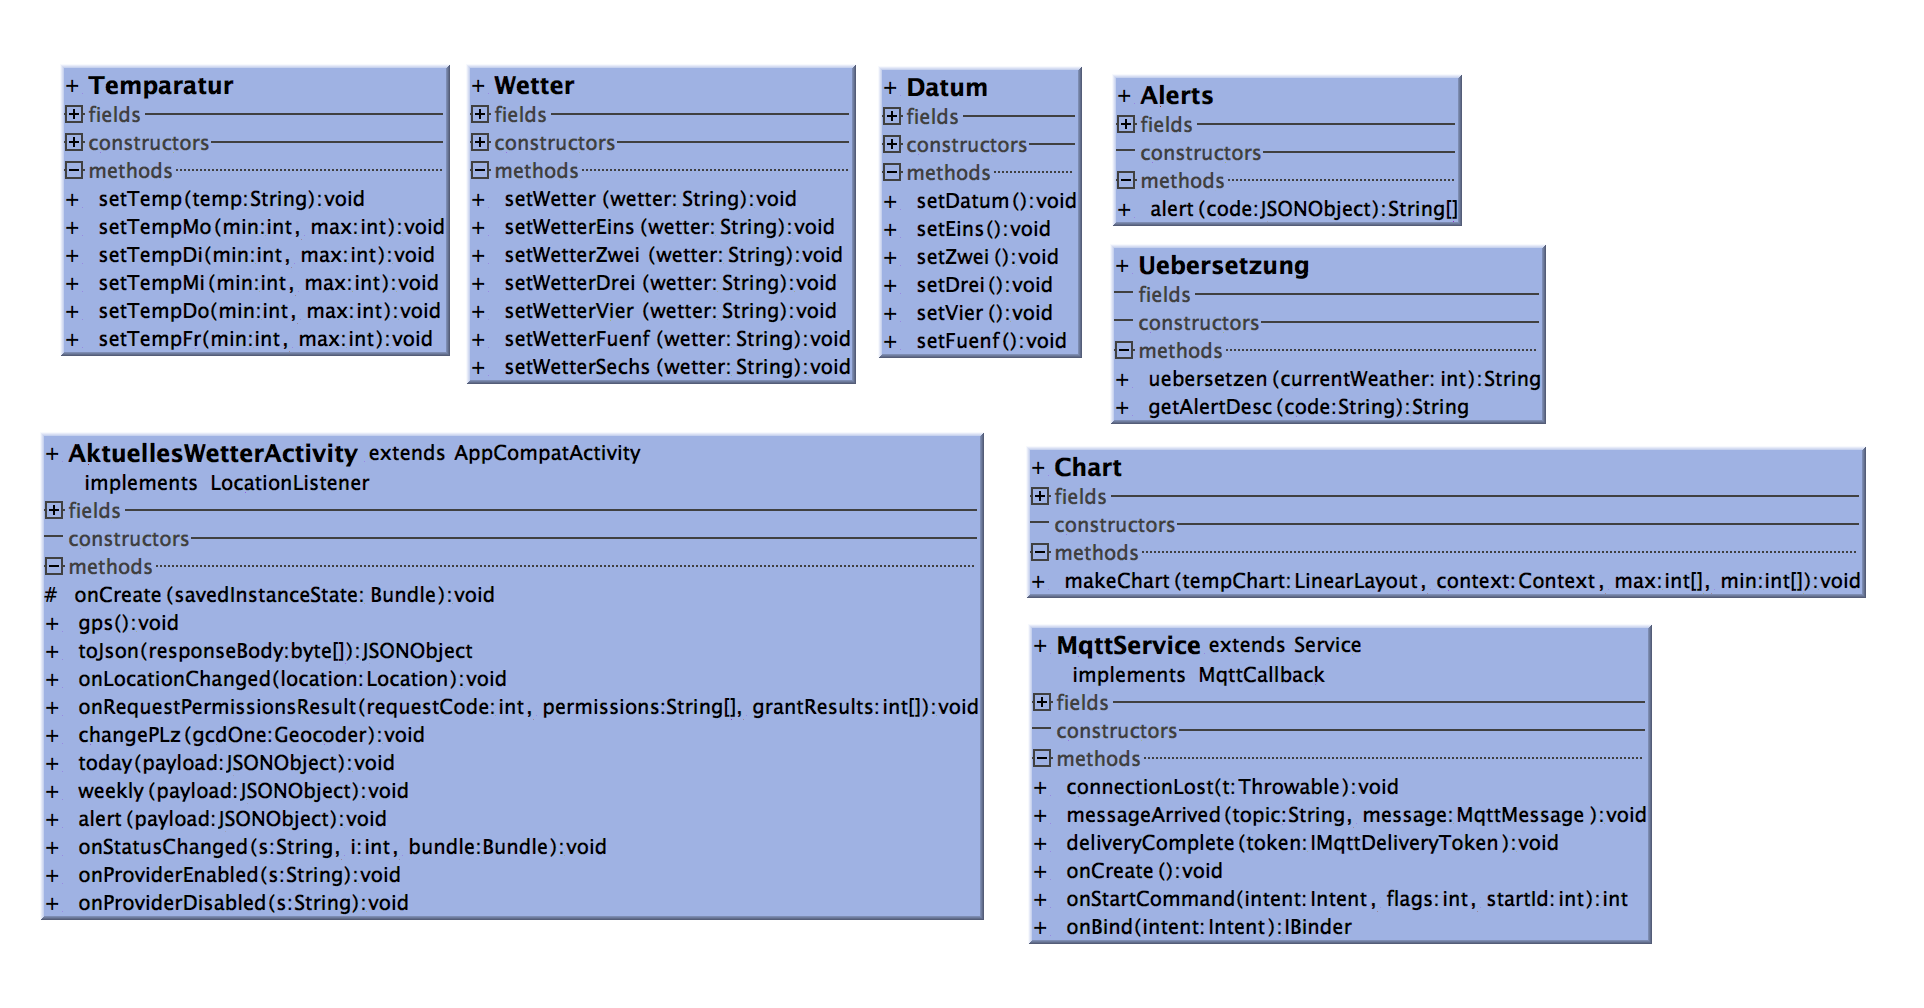
\includegraphics[width=0.5\textwidth]{Bilder/AndroidUML.png}
	\caption{Klassendiagramm der Android-Applikation}
	\label{img:AndroidUMLDiagramm}
\end{figure} 
Die Applikation wurde in Androidstudio in der Sprache Java und XML geschrieben. 
Aufgebaut ist die Applikation über 8 Klassen wie in (Siehe Abb. \ref{img:AndroidUMLDiagramm})

\subsection{Web-Client}